\documentclass[11pt,a4paper]{article}
\usepackage[utf8]{inputenc}
\usepackage[french]{babel}
\usepackage[T1]{fontenc}
\usepackage{amsmath}
\usepackage{amsfonts}
\usepackage{amssymb}
\usepackage{graphicx}
\usepackage[left=2cm,right=2cm,top=2cm,bottom=2cm]{geometry}
\usepackage{verbatim} 
\author{Malika NEDJAR}
\title{document technique}
\begin{document}

\section{ Introduction}

L'installation et le paramétrage de ELK (Elasticsearch, Logstash et Kibana) sur un serveur "loghost-ng" et sans installation de Logstash Forwarder (appelé auparavant Lumberjack) sur les machines clientes dont nous souhaitons analyser les logs car les logs sont centralisé au niveau de serveur. Le serveur Web sera le serveur apache.

La récupération des logs est centralisée avec les outils rsyslog et Logstash qui est un excellent produit de tri, traitement et collecte des logs.

Le logiciel logstash possède de nombreux avantages, entres autres:

\begin{itemize}
\item Il est compatible avec les protocoles courants comme syslog, idéal pour s'insérer dans des architectures existantes. 
\item Il est extensible dans le sens où tout est configuré en utilisant des expressions régulières, dont beaucoup sont déjà fournies.
\item Il est très scalable car il repose sur une base de données elasticsearch (qui peut fonctionner en cluster), des services de "cache" (broker). 
\end{itemize}

Pour la mise en oeuvre au sein d'une architecture simple, logstash se positionne sur un serveur central faisant office de collecteur de logs. Sur ce serveur logstash est configuré avec une entrée de type syslog sur le port 5000 (par ex).

\section{ Installation de ELK}
ELK : Il s'agit de la combinaison de trois logiciels : \textbf{Elasticsearch} en tant que moteur d'indexation, \textbf{Logstash} pour la collecte, l’analyse et le stockage de logs, et \textbf{Kibana} pour construire des graphiques et requêter et visualiser n'importe quelles données. L'ensemble étant assez complet.
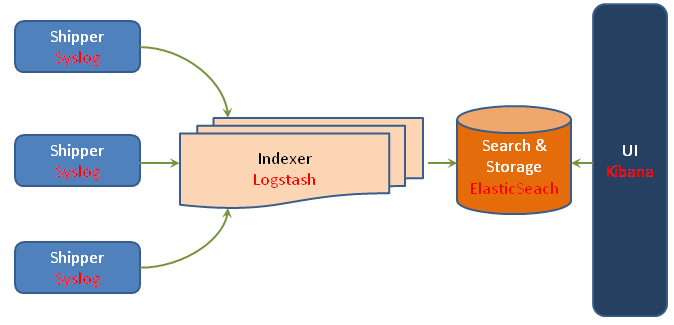
\includegraphics[scale=0.5]{image.png} 
\subsection{Installation de Elasticsearch}
Elasticsearch est le moteur de recherche open source rendu populaire avec l'arrivée du big data. Il propose des fonctionnalités avancées, facilement configurable, rivalisant avec les meilleurs logiciels propriétaires. Un moteur de recherche, c'est une brique technologique capable d'ingérer un nombre massif de données, et de les mettre à disposition d'un utilisateur de façon intelligente, en quelques millisecondes. 
 \begin{verbatim}
$wget -qO - https://packages.elastic.co/GPG-KEY-elasticsearch | sudo apt-key add -
$echo "deb http://packages.elastic.co/elasticsearch/1.5/debian stable main" | 
 sudo tee -a /etc/apt/sources.list
$sudo apt-get update && sudo apt-get install elasticsearch
 \end{verbatim}
Après on modifie quelques champs dans le fichier  \textbf{/etc/default/elasticsearch} et en redémarre Elasticsearch.

\begin{verbatim}
# Elasticsearch log directory
LOG_DIR=/var/log/elasticsearch

# Elasticsearch data directory
DATA_DIR=/var/lib/elasticsearch

# Elasticsearch work directory
WORK_DIR=/tmp/elasticsearch
https://www.youtube.com/watch?v=Rbsg5QWqvPM
# Elasticsearch configuration directory
CONF_DIR=/etc/elasticsearch

# Elasticsearch configuration file (elasticsearch.yml)
CONF_FILE=/etc/elasticsearch/elasticsearch.yml
\end{verbatim}

ElasticSearch est maintenant installé. on passe à la configuration d'Elasticsearch, en éditant le fichier de configuration, /etc/elasticsearch/elasticsearch.yml, et modifier les éléments suivants:


\begin{itemize}
\item Remplacer la ligne \textbf{\#network.host: 192.168.0.1} par \textbf{network.host: loghost-ng}
\item Décommenter la ligne \textbf{\#cluster.name: elasticsearch} 
\item Remplacer la ligne \textbf{\#node.name: “Franz Kafka”} par \textbf{node.name: cremi}
\item Décommenter la ligne \textbf{\#node.master: true}
\item Décommenter la ligne \textbf{\#node.data: true}
\item Décommenter la ligne \textbf{\#discovery.zen.ping.multicast.enabled: false}
\item Remplacer la ligne \textbf{\#index.number\_of\_shards: 5} par \textbf{index.number\_of\_shards: 1}
\item Remplacer la ligne \textbf{\#index.number\_of\_replicas: 1} par \textbf{index.number\_of\_replicas: 0}

\end{itemize}

Après avoir configurer Elasticsearch, on active le service elasticsearch:

\begin{verbatim}
$systemctl daemon-reload
$systemctl enable elasticsearch.service
$service elasticsearch restart
\end{verbatim}

Ensuite, on exécute la commande suivante pour démarrer Elasticsearch au démarrage:

\begin{verbatim}
$sudo update-rc.d elasticsearch defaults 95 10
\end{verbatim}

On vérifie qu'ElasticSearch s'est correctement lancé consiste à ouvrir l'URL\textit{ \textbf{http://loghost-ng:9200/}} dans un navigateur Web. En effet, ElasticSearch écoute par défaut sur le port 9200 pour répondre aux éventuelles requêtes HTTP REST qui lui sont faites.
La réponse du serveur confirme le bon fonctionnement d'ElasticSearch et rappelle le numéro de la version installée :
\begin{verbatim}
# curl 'http://loghost-ng:9200/_search?pretty'
ou
# curl 'http://loghost-ng:9200/_nodes/?pretty'
\end{verbatim}

\subsection{Installation de logstash}
Logstash est un outil de collecte, analyse et stockage de logs. Pour la collecte, il sait gérer plus d'une trentaine d'événements. Un événement peut être un message syslog, un mail via le protocole IMAP, un tweet ou encore une commande IRC.

Il va ensuite analyser ces événements, et les mettre en forme à l'aide de filtres. Il existe également une vingtaine de filtres : standardisation de la date, découpage du message, structuration du message via grok.
Après filtrage, on obtient un message relativement clair, avec des couples clé-valeur que l'on pourra exploiter plus tard.

Enfin, il exporte ces données, traitées ou non, sous divers formats : email, sortie standard, fichier texte, alarme Nagios, entrée en base de données ElasticSearch.

Ainsi, on peut très bien traiter plusieurs flux de logs différents, appliquer un filtre à chacun pour harmoniser le tout, et les stocker correctement.

Logstash utilise Java, il est donc nécessaire qu’un JDK soit installé sur le “serveur”. On peut utiliser au choix OpenJDK ou Oracle JDK.

\begin{verbatim}
$wget -qO - http://packages.elasticsearch.org/GPG-KEY-elasticsearch | sudo apt-key add -
$deb http://packages.elasticsearch.org/logstash/1.4/debian stable main
$echo 'deb http://packages.elasticsearch.org/logstash/1.4/debian stable main' | 
 sudo tee /etc/apt/sources.list.d/logstash.list
$apt-get update
$apt-get install logstash
 
$curl 'http://loghost-ng:9200/'
$service logstash start 
\end{verbatim}
Dans mon installation, les fichiers de configuration se trouvent dans le dossier \textbf{/etc/logstash/conf.d}.

Dans ma configuration j’utilise deux types d’entrées :
\begin{itemize}
    \item Des entrées de types fichiers, créés par le rsyslog serveur.
    \item Des entrées de type syslog qui agissent comme un serveur syslog qui écoute.
\end{itemize}

Pour la partie “input” du serveur, on crée le fichier \textbf{input.conf} ou j'ai choisis les entrées de type syslog qui agissent comme un serveur syslog qui écoute sur le port 5000 et pour celà, j'ai configuré \textbf{rsyslog} pour qu'il envois tous les logs ver le port 5000 en créant le fichier \textbf{/etc/rsyslog.d/logstash.conf}:
\begin{verbatim}
$template LOGSTASH,"<%PRI%>%TIMESTAMP% %HOSTNAME% %syslogtag%%msg%"
$ActionForwardDefaultTemplate LOGSTASH
*.* @@10.0.220.22:5000
\end{verbatim}
voici le fichier \textbf{input.conf}.
\begin{verbatim}
input {
        syslog {
                port => 5000
                host => "0.0.0.0"
                type => "syslog"
        }

#       file {
#               path => ["/srv/log/*.log", "/srv/log/syslog"]
#               exclude => "*.gz"
#                type => "syslog"
#       }
}
\end{verbatim}

Pour la partie “input” du serveur, on crée le fichier \textbf{filter.conf}.

\begin{verbatim}
filter {
if [type] == "syslog" {
        grok {
        	match => { "message" => "<%{POSINT:syslog_pri}>%
        	{SYSLOGTIMESTAMP:timestamp} 
        	%{SYSLOGHOST:logsource} %{DATA:program}(?:\
        	[%{POSINT:syslog_pid}\])?: %{GREEDYDATA:message}" }
        	
        	overwrite => [ "%{[logsource]}" ]			
        	add_field => [ "received_at", "%{@timestamp}" ]
        	add_field => [ "received_from","%{logsource}" ]
        }
        syslog_pri { }

        date {
        	 match => [ "timestamp", "MMM  d HH:mm:ss", "MMM dd HH:mm:ss" ]
        }
}
if [program] == "pperso-access" {
	grok {
      	 # logs HTTPS 
      	 match => { "message" => "%{COMBINEDAPACHELOG}  %{IPORHOST:host} %
      	 {GREEDYDATA:ssl_protocol} %{GREEDYDATA:ssl_cipher}"}
       	 # logs HTTP
       	 match => { "message" => "%{COMBINEDAPACHELOG}  %{IPORHOST:host}" }
    }
	mutate {
        replace => ["type","apache"]
       	}

	useragent { 
      	prefix => "agent." 
      	source => "agent" 
    	}
# Add geolocalization attributes based on ip.
	geoip { 
      		source => "clientip" 
      		target => "geoip" 
      		database => "/usr/share/GeoIP/GeoLiteCity.dat" 
      		add_field => [ "[geoip][coordinates]", "%{[geoip][longitude]}" ] 
      		add_field => [ "[geoip][coordinates]", "%{[geoip][latitude]}"  ] 
    	} 
	mutate {
      		convert => [ "[geoip][coordinates]", "float" ]
      		gsub => [
        		"referrer", "^\"", "",
        		"referrer", "\"$", "",
        		"agent", "^\"", "",
        		"agent", "\"$", ""
      		]
	} 
}
#On reforme le message avec les infos sélectionnées
#  	mutate { 
#     		replace => ["host","%{logsource}"]
# 		replace => [ "host", "%{hostname}" ]
#  	}
}









\end{verbatim}

Pour la partie “output” du serveur, on crée le fichier \textbf{output.conf}.
\begin{verbatim}
output {
  elasticsearch {
    protocol => "http"
    flush_size => '100'
    host => 'loghost-ng'
    index => 'logstash-%{+YYYY.MM.dd}'
    port => '9200'
  }
# just pour débuger /srv/log/logstash/logstash.stdout
    stdout {
       codec => rubydebug
    }
}
\end{verbatim}

\subsection{Installation de Kibana}
Kibana est une interface web permettant de rechercher des informations stockées par Logstash dans ElasticSearch.

\begin{verbatim}
$cd /opt
$wget https://download.elasticsearch.org/kibana/kibana/kibana-4.0.1-linux-x64.tar.gz

$tar xvf kibana-*.tar.gz
$vi /opt/kibana/config/kibana.yml
$cd /etc/init.d && sudo wget https://gist.githubusercontent.com/thisismitch/
 8b15ac909aed214ad04a/raw/bce61d85643c2dcdfbc2728c55a41dab444dca20/kibana4

$sudo chmod +x /etc/init.d/kibana4
$sudo update-rc.d kibana4 defaults 96 9
$sudo service kibana4 start

$systemctl enable kibana
$systemctl start kibana
\end{verbatim}

apres l'installation on passe à la configuration de kinana, en éditant 
sur le navigateur 
En effectuant des requêtes qui permettent de retrouver parmi tous les logs les connexions (les authentifications) voici quelques requêtes:
La requête pour visualiser tous les connexions:
\begin{verbatim}
"(kdm:session)" AND "session opened for user"
ou
"session opened for user" AND kdm NOT "session opened for user nagios" NOT
 "session opened for user root" NOT "session opened for user fberarde" NOT
  "session opened for user netdb" NOT "session opened for user www-data"
\end{verbatim}
La requête pour visualiser tous les connexions de la salle 001 \& 004:
\begin{verbatim}
"(kdm:session)" AND "session opened for user" AND 10.0.4.*
\end{verbatim}
La requête pour visualiser tous les connexions de la salle 101:
\begin{verbatim}
"(kdm:session)" AND "session opened for user" AND 10.0.101.*
\end{verbatim}
\end{document}